\chapter{Linear Array and Ring Networks}

The \textbf{linear array} and the \textbf{ring} are interconnection networks of processors organized in the shape of a ``line''. Each processor is physically linked only to each of its neighbours, which in the linear array can either be two or just one for the outmost processors, instead in the ring they are always two, since processors are connected in a circle. Examples, with $P = 6$ processors, of both kinds of networks are depicted below. 

\begin{itemize}

\item \textbf{linear array}: links are \bfit{bidirectional}, indicated by the straight lines. 

\begin{figure}[H]
    \centering
    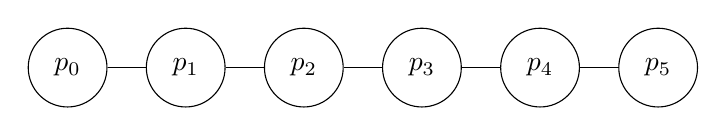
\begin{tikzpicture}[every node/.style={draw, circle, minimum size=1cm, inner sep=0pt}]
        \node (p0) at (0,0) {$p_0$};
        \node (p1) at (1.5,0) {$p_1$};
        \node (p2) at (3,0) {$p_2$};
        \node (p3) at (4.5,0) {$p_3$};
        \node (p4) at (6,0) {$p_4$};
        \node (p5) at (7.5,0) {$p_5$};
        \foreach \i/\j in {p0/p1, p1/p2, p2/p3, p3/p4, p4/p5}
            \draw[-] (\i) -- (\j);
    \end{tikzpicture}
    \caption{Linear array with 6 processors and bidirectional links.}
    \label{fig:linear-array}
\end{figure}

\vspace{-1em}

\item \textbf{ring}: links are \bfit{unidirectional}, in which case they are represented using arrows, to specify the direction in which data can flow.

\begin{figure}[H]
    \centering
    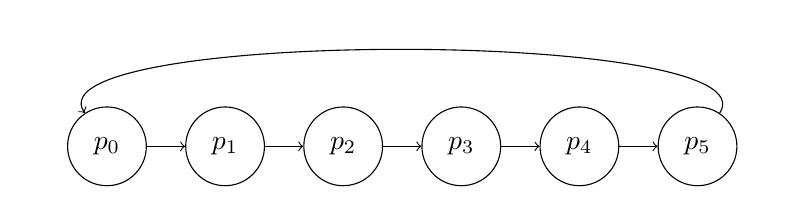
\begin{tikzpicture}[every node/.style={draw, circle, minimum size=1cm, inner sep=0pt}]
        \node (p0) at (0,0) {$p_0$};
        \node (p1) at (1.5,0) {$p_1$};
        \node (p2) at (3,0) {$p_2$};
        \node (p3) at (4.5,0) {$p_3$};
        \node (p4) at (6,0) {$p_4$};
        \node (p5) at (7.5,0) {$p_5$};
        \foreach \i/\j in {p0/p1, p1/p2, p2/p3, p3/p4, p4/p5}
        \draw[->] (\i) -- (\j);
        \draw[->] (p5) .. controls (8.5,1.5) and (-1,1.5) .. (p0);
    \end{tikzpicture}
    \caption{Ring with 6 processors and unidirectional links.}
    \label{fig:ring}
\end{figure}

\vspace{-1em}

\end{itemize}

The number of processors and the kind of links adopted will be specified for each network depending on the use case.

\subsubsection{Properties}

\vspace{-0.5em}

\begin{multicols}{2}
\begin{center}
\textbf{Linear array}
\end{center}

\begin{itemize}
    \item \bfit{Diameter} $diam(L_P) = P-1$, i.e., the distance between the two opposite outmost processors.
    \item \bfit{Bisection bandwidth} $b(L_P) = 1$, independent of the number $P$ of processors.
\end{itemize}

\columnbreak

\begin{center}
\textbf{Ring} 
\end{center}

\begin{itemize}
    \item \bfit{Diameter} $diam(R_P) = \lfloor P/2 \rfloor$, i.e., the maximum distance between two processors.
    \item \bfit{Bisection bandwidth} $b(R_P) = 2$, independent of the number $P$ of processors.
\end{itemize}
\end{multicols}

\section{Odd-Even Transposition Sort}

The \textbf{odd-even transposition sort} is a simple sorting algorithm that can be implemented on a linear array. Given $N$ values, each in input to a different processing unit of a linear array with $P = N$, constant memory $M = 1$ and bidirectional links, the task will take at least $N-1$ steps, since in the worst case it requires to move the value initially in the leftmost processor to the rightmost one, or the opposite. Despite being very simple, odd-even transposition sort is actually very efficient, because it always takes exactly $N$ steps, so just one more than the previous lower bound.

The algorithm proceeds through $N$ steps, where at each step $t = 0 \ldots N-1$, processors with indices matching the parity of $t$ (i.e., both even or both odd) engage in comparison and potential value exchange with their right neighbor. Specifically, processor $i$ compares its value with processor $i+1$'s value (if $i+1 < N$ exists) and swaps them if necessary to maintain ascending order. Each processor makes its decision based on its known index position in the linear array. This process continues until step $N-1$, at which point all values are guaranteed to be sorted in ascending order across the processor array.

\begin{figure}[H]
    \centering
    \begin{tikzpicture}[every node/.style={draw, minimum size=0.8cm, font=\small}, node distance=1.2cm]
        % Step 1
        \node (a1) at (0,0) {4};
        \node (a2) [right=of a1] {3};
        \node (a3) [right=of a2] {1};
        \node (a4) [right=of a3] {2};
        % Arrows for step 1
        \draw[<->,thick] (a1) -- (a2);
        \draw[<->,thick] (a3) -- (a4);
        % Step label
        \node[draw=none, right=0.5cm of a4, align=left] (l1) {step 1};

        % Step 2
        \node (b1) at (0,-1.5) {3};
        \node (b2) [right=of b1] {4};
        \node (b3) [right=of b2] {1};
        \node (b4) [right=of b3] {2};
        % Arrows for step 2
        \draw[<->,thick] (b2) -- (b3);
        % Step label
        \node[draw=none, right=0.5cm of b4, align=left] (l2) {step 2};

        % Step 3
        \node (c1) at (0,-3) {3};
        \node (c2) [right=of c1] {1};
        \node (c3) [right=of c2] {4};
        \node (c4) [right=of c3] {2};
        % Arrows for step 3
        \draw[<->,thick] (c1) -- (c2);
        \draw[<->,thick] (c3) -- (c4);
        % Step label
        \node[draw=none, right=0.5cm of c4, align=left] (l3) {step 3};

        % Step 4
        \node (d1) at (0,-4.5) {1};
        \node (d2) [right=of d1] {3};
        \node (d3) [right=of d2] {2};
        \node (d4) [right=of d3] {4};
        % Arrows for step 4
        \draw[<->,thick] (d2) -- (d3);
        % Step label
        \node[draw=none, right=0.5cm of d4, align=left] (l4) {step 4};

        % Connectors (lines between nodes)
        \foreach \i/\j in {a1/a2, a2/a3, a3/a4, b1/b2, b2/b3, b3/b4, c1/c2, c2/c3, c3/c4, d1/d2, d2/d3, d3/d4}
            \draw[-] (\i) -- (\j);
    \end{tikzpicture}
    \caption{Odd-even transposition sort computation on a linear array with $P=N=4$.}
    \label{fig:odd-even-example}
\end{figure}

\vspace{-1em}

Odd-even transposition sort belongs to a class of sorting algorithms called \bfit{oblivious comparison-exchange algorithms}. The comparison-exchange part means simply that the algorithms operates only by comparing pairs of values and possibly exchanging their positions. On the other hand, \bfit{oblivious} means that the behaviour of the algorithm does not depend on the input values, that is, the algorithm always performs the same sequence of comparison-exchange operations, on predetermined pairs, independently on the values to be sorted. To prove the correctness of this kind of sorting algorithms we can use the following lemma.

\rule{\textwidth}{0.4pt}
\begin{Lemma}[0-1 sorting]

    \phantom{c}

    If an oblivious comparison-exchange algorithm sorts all input sets consisting solely of 0s and 1s, then it sorts all input sets with arbitrary values.
\end{Lemma}

\vspace{-1em}

\hdashrule{\textwidth}{0.1pt}{2mm 1.5mm}

\vspace{-0.5em}

\begin{proof}[\textbf{Proof}] \renewcommand{\qedsymbol}{$q.e.d.$}

    Assume by contradiction that the algorithm fails to sort some sequence of arbitrary values $x_0, x_1, \ldots, x_n$. Let $\pi$ be a permutation such that $x_{\pi(0)}, x_{\pi(1)}, \ldots, x_{\pi(n)}$ is the output of the algorithm. Since the algorithm fails to sort the sequence, there must exist a pair of indices $h$ and $k$ such that $h < k$ but $x_{\pi(h)} > x_{\pi(k)}$. Now, for every $0 \leq i \leq n$ define
    $$
        y_i = \begin{cases}
            0 & \text{if } x_i \leq x_{\pi(k)} \\
            1 & \text{if } x_i > x_{\pi(k)}
        \end{cases}
    $$
    Observe that, for every $i$ and $j$, if $x_i \leq x_j$ then also $y_i \leq y_j$, because otherwise we would have $x_i \geq x_{\pi(k)} \geq x_j \geq x_i$. Therefore, the algorithm, being oblivious and comparison-based, would perform exactly the same exchanges when executed on either sequence, resulting in the same permutation $\pi$ of before and output $y_{\pi(0)}, y_{\pi(1)}, \ldots, y_{\pi(n)}$. Since we know that $x_{\pi(h)} > x_{\pi(k)}$, then $y_{\pi(h)} = 1$ and clearly $y_{\pi(k)} = 0$. But since $h < k$, this contradicts the hypothesis that the algorithm correctly sorts all inputs with only 0s and 1s.
\end{proof}
\vspace{-1.2em}

\rule{\textwidth}{0.4pt}

\newpage

Using the previous lemma, in order to prove correctness of an oblivious comparison-exchange algorithm, it is enough to show that it can sort all inputs consisting of solely 0s and 1s.

For instance, in the case of odd-even transposition sort, let the input be any sequence of $k$ 1s and $N-k$ 0s, in some order. We need to show that, within $N$ steps, the 1s have all been moved to the $k$ rightmost processors, that is, those indexed by $N-k, N-k+1, \ldots, N-1$. Observe that after any comparison performed between two adjacent processors, a 1 can only move to the right, or not move at all. Let $k$ be the rightmost processor to initially have a 1. Then, all processors to its right will have 0s (since we have $k$ 1s initially). So, depending on the parity of $h$, during either the first or the second step of the computation the rightmost 1 will start moving to the right, and it will continue doing so at every subsequent step until it reaches the last processor $N-1$. This also means that shortly after the second step, so at least from the third, the second rightmost 1 will also start moving to the right and will only stop once it reaches processor $N-2$. This reasoning extends to all the $k$-th step: in general, the $i$-th rightmost 1 will move at most $i$ steps, after which it will start moving to the right and continue doing so until it reaches processor $N-i$. 

Note that the $i$-th rightmost 1 initially can at most be located in processor $k-i$, which is distant $N-k$ from its final destination, that is, processor $N-i$. So, all is need to move at most $N-k$ times. Furthermore, since each of them will stay still for at most $k$ steps, and will move at every step after that, this means that within $k + N - k = N$ steps all 1s will have reached their destination, and the sequence will, in fact, be sorted.

\subsection*{Performances}

\begin{itemize}
    \item The \textbf{parallel execution time} is $T_{N}(N) = \Theta(N)$, since the procedure takes exactly $N$ steps. The total \textbf{work} performed is $W = \Theta(N^2)$, as each of the $N$ processors performs $\Theta(N)$ operations.
    \item The \textbf{speedup} is $S = \Theta(N \log N)/\Theta(N) = \Theta(\log N)$ when compared to the fastest sequential sorting algorithm. Consequently, the \textbf{efficiency} is $\varepsilon = \Theta\left(\frac{\log N}{N}\right)$, indicating that the parallel implementation becomes less efficient as $N$ grows.
\end{itemize}

\section{Ranked Enumeration Sort}

A different kind of sorting algorithms, counts for each value to be sorted how many precede it in the order. Clearly, these are not comparison-exchange algorithms. A simple algorithm of this kind is \textbf{rank enumeration sort}, meant to execute on a ring with $P = N$ processing units with constant memory $M = 2$, working as follows:

\begin{itemize}
    \item The values, initially assigned each one to a different processing unit, are circulated around the ring, together with the index of their initial processor.
    \item Every time a processing unit $i$ receives a pair $(x_j, j)$, it adds 1 to its own counter $r_i$ only if $x_j < x_i$, or if $x_j = x_i$ and $j < i$. Indeed, the order which is actually used is the so-called lexicographic order on the pairs (value, index).
    \item Since every index is unique, there can be no duplicates among the pairs.
    \item After every processor $i$ had opportunity to see every other value, i.e.\ after $N-1$ steps, its counter $r_i$ will be the rank of the value $x_i$ that it originally received. So, the rank $r_i$ is the number of values that precede $x_i$ once the sequence is sorted, which is also the index of the processor where $x_i$ should be at the end.
    \item Then, the pairs $(x_i, r_i)$ stored in each processor $i$ are circulated around the ring, before for another $N-1$ steps. This way, when processor $r_i$ receives the pair $(x_i, r_i)$, matching its own index, it will simply hold onto and store the value $x_i$, while continuing passing along all the others.
\end{itemize}

Thus we said once before about the lexicographic order, this method will distribute all values to their $2N-2$ total steps to obtain the sorted order. Note also that unidirectional links are enough to execute this algorithm.

\subsubsection{Performances}

\begin{itemize}
    \item The \textbf{parallel execution time} is $T_{N}(N) = \Theta(N)$ since the procedure takes exactly $2N-2$ constant steps, then the work is $W = \Theta(N^2)$.
    \item The \textbf{speedup} is $S = \Theta(N \log N)/\Theta(N) = \Theta(\log N)$ w.r.t. the fastest sequential sorting algorithm, hence the efficiency is $\varepsilon = \Theta\left(\frac{\log N}{N}\right)$.
\end{itemize}

\section{Discrete Convolution}

The \textbf{discrete convolution} of two $N$-vectors $\vec{a} = (a_0, \ldots, a_{N-1})$ and $\vec{b} = (b_0, \ldots, b_{N-1})$ is the $(2N-1)$-vector $\vec{c} = (c_0, \ldots, c_{2N-2})$ where $c_k$, for every $0 \leq k \leq 2N-2$, is defined by
$$
    c_k = \sum_{\substack{0 \leq i, j < N}}^{i + j = k} a_i b_j,
$$
i.e., the sum of products of elements with indices that sum to $k$. Convolutions arise in a variety of applications, including signal processing and polynomial multiplication.

In order to compute every $c_k$ on a systolic linear array with $P = 2N$ and $M = 1$, we need to find a flow of the data such that, for every $i$ and $j$, the values $a_i$ and $b_j$ meet, simultaneously, during the same step at the processing unit computing $c_{i+j}$. This ensures that each component of each sum is accounted for in the right place, and that the constant memory space is not exceeded in the process.

One way to do this is to input data one value at a time from both ends of the linear array, $\vec{a}$ from the right and $\vec{b}$ from the left, and make them flow towards the opposite direction. Furthermore, to guarantee that all pairs correctly align with the corresponding processing units, the values are input in alternating orders: the first value of $\vec{a}$ at the end of $\vec{a}$ and $\vec{b}$ is input in reverse order $b_{N-1}, \ldots, b_0$, while $\vec{a}$ in the regular one.

The flow of data for the computation of the discrete convolution of two vectors of size $N=3$ is shown in Figure~4. The computation of each $c_k$ is done entirely by processing unit $k$, which updates its $c_k = c_k + a_i b_j$ every time it receives values $a_i, b_j$ from both sides during the same step. Initially, $c_k = 0$ in every processor $k$.

As can be seen in the figure, each value $a_i$ enters the linear array from the right at step $2i+1$, and then moves one to the left at every subsequent step. Therefore value $a_i$ will be located in processor $k$ at step $2i+2N-k$.

\subsubsection*{Performances}

\begin{itemize}
    \item The \textbf{parallel execution time} is $T_{2N}(N) = \Theta(N)$ since the procedure takes exactly $3N-1$ constant steps, then the work is $W = \Theta(N^2)$.
    \item The \textbf{speedup} is $S = \Theta(N^2)/\Theta(N) = \Theta(N)$ w.r.t. naive sequential algorithms which would compute the product of each pair $a_i, b_j$; in such a case the efficiency is $\mathcal{E} = \Theta\left(\frac{N}{2N}\right) = \Theta(1)$, while the latter is not that informative it highlights that it is actually bounded by a constant, independent of $N$.
\end{itemize}